\documentclass[aps,prb,twocolumn,superscriptaddress,floatfix,longbibliography]{revtex4-2}

\usepackage[utf8]{inputenc}
\usepackage[spanish]{babel}
\usepackage{graphicx}
\usepackage{amsmath}
\usepackage{subcaption}
\usepackage{wrapfig} 
\usepackage[export]{adjustbox}

\usepackage{amsmath,amssymb} % math symbols
\usepackage{bm} % bold math font
\usepackage{graphicx} % for figures
\usepackage{comment} % allows block comments
\usepackage{textcomp} % This package is just to give the text quote '
\usepackage{listings} %para agregar código

%\usepackage{ulem} % allows strikeout text, e.g. \sout{text}

\usepackage[spanish]{babel}

\usepackage{enumitem}
\setlist{noitemsep,leftmargin=*,topsep=0pt,parsep=0pt}

\usepackage{xcolor} % \textcolor{red}{text} will be red for notes
\definecolor{lightgray}{gray}{0.6}
\definecolor{medgray}{gray}{0.4}

\usepackage{hyperref}
\hypersetup{
colorlinks=true,
urlcolor= blue,
citecolor=blue,
linkcolor= blue,
bookmarks=true,
bookmarksopen=false,
}

% Code to add paragraph numbers and titles
\newif\ifptitle
\newif\ifpnumber
\newcounter{para}
\newcommand\ptitle[1]{\par\refstepcounter{para}
{\ifpnumber{\noindent\textcolor{lightgray}{\textbf{\thepara}}\indent}\fi}
{\ifptitle{\textbf{[{#1}]}}\fi}}
%\ptitletrue  % comment this line to hide paragraph titles
%\pnumbertrue  % comment this line to hide paragraph numbers

% minimum font size for figures
\newcommand{\minfont}{6}

% Uncomment this line if you prefer your vectors to appear as bold letters.
% By default they will appear with arrows over them.
% \renewcommand{\vec}[1]{\bm{#1}}

%Cambiar Cuadros por Tablas y lista de...
%\renewcommand{\listtablename}{Índice de tablas}
\renewcommand{\tablename}{Tabla}
\renewcommand{\date}{Fecha}

% \graphicspath{ {C:/Users/lupam/Mi unidad/Pablo Chehade/Instituto Balseiro (IB)/Laboratorio Avanzado/Informe/V5/Figures} } %Para importar imagenes desde una carpeta


\lstset{
  basicstyle=\ttfamily\small,
  breaklines=true,
  frame=single,
  numbers=left,
  numberstyle=\tiny,
  keywordstyle=\color{blue},
  commentstyle=\color{green},
  stringstyle=\color{red},
} %Configuración para el bloque de código


\usepackage[bottom]{footmisc} %para que las notas al pie aparezcan en la misma página



\begin{comment}

%Comandos de interes:

* Para ordenar el documento:
\section{Introducción}
\section{\label{sec:Formatting}Formatting} %label para luego hacer referencia a esa sección

\ptitle{Start writing while you experiment} %pone nombre y título al documento dependiendo de si en el header están los comandos \ptitletrue y \pnumbertrue

* Ecuaciones:
\begin{equation}
a^2+b^2=c^2 \,.
\label{eqn:Pythagoras}
\end{equation}

* Conjunto de ecuaciones:
\begin{eqnarray}
\label{eqn:diagonal}
\nonumber d & = & \sqrt{a^2 + b^2 + c^2} \\
& = & \sqrt{3^2+4^2+12^2} = 13
\end{eqnarray}

* Para hacer items / enumerar:
\begin{enumerate}
  \item
\end{enumerate}

\begin{itemize}
  \item
\end{itemize}

* Figuras:
\begin{figure}[h]
    \includegraphics[clip=true,width=\columnwidth]{pixel-compare}
    \caption{}
     \label{fig:pixels}
\end{figure}

* Conjunto de figuras:
(no recuerdo)


* Para hacer referencias a fórmulas, tablas, secciones, ... dentro del documento:
\ref{tab:spacing}

* Para citar
Elementos de .bib
\cite{WhitesidesAdvMat2004}
url
\url{http://www.mendeley.com/}\\

* Agradecimientos:
\begin{acknowledgments}
We acknowledge advice from Jessie Zhang and Harry Pirie to produce Fig.\ \ref{fig:pixels}.
\end{acknowledgments}

* Apéndice:
\appendix
\section{\label{app:Mendeley}Mendeley}

* Bibliografía:
\bibliography{Hoffman-example-paper}

\end{comment}



\begin{document}

% Allows to rewrite the same title in the supplement
\newcommand{\mytitle}{Dinámica de sistemas acoplados}

\title{\mytitle}

\author{Pablo Chehade \\
    \small \textit{pablo.chehade@ib.edu.ar} \\
    \small \textit{Redes Neuronales, Instituto Balseiro, CNEA-UNCuyo, Bariloche, Argentina, 2023} \\}
    
    
    
\maketitle



\section{Ejercicio 1}
Se analizó la interacción entre dos neuronas Hodgkin-Huxley idénticas conectadas simétricamente con interacciones sinápticas excitatorias. La dinámica de cada neurona se describe mediante el sistema de ecuaciones diferenciales:

\begin{equation}
\left\{\begin{array}{@{}l@{}}
    C \frac{dV}{dt} = I_{ext} + I_{syn,pre} - g_{Na}m^3h(V-V_{Na}) \\ 
    \hspace{4em} - g_{K}n^4(V - V_k) - g_l(V-V_l)    \\
    \frac{dm}{dt} = (m_\infty(V) - m)/\tau_m(V)    \\
    \frac{dh}{dt} = (h_\infty(V) - h)/\tau_h(V)    \\
    \frac{dn}{dt} = (n_\infty(V) - n)/\tau_n(V)    \\
    \frac{ds}{dt} = (s_\infty(V_{pre}) - s)/\tau_s,
    \end{array}\right.
    \label{eq:ej1_ecs_difs}
\end{equation}

donde $x_\infty(V) = a_x/(a_x + b_x)$ y $\tau_x(V) = 1/(a_x + b_x)$ para $x = m, h, n$. Las funciones $a_x$ y $b_x$ se definen como:
\[
\left\{\begin{matrix}
    a_m = 0.1(V + 40)/(1 - e^{-(V+40)/10}) \\
    b_m = 4 e^{- (V + 65)/18}    \\
    a_h = 0.07 e^{- (V+65)/20} \\ 
    b_h = 1/(1 + e^{- (V+35)/10})    \\
    a_n = 0.01(V+55)/(1-e^{-(V+55)/10}) \\
    b_n = 0.125 e^{-(V+65)/80}.
    \end{matrix}\right.
\]
Además, $s_\infty = 0.5 (1 + \tanh(V/5))$ y $\tau_s = 3$ ms.

Los valores de potenciales de inversión y conductancias máximas son: $V_{Na} = 50$ mV, $V_K = -77$ mV, $V_l = -54.4$ mV, $g_{Na} = 120$ $\mathrm{mS/cm^2}$, $g_K = 36$ $\mathrm{mS/cm^2}$, $g_l = 0.3$ $\mathrm{mS/cm^2}$. La capacitancia de membrana es $C = 1$ $\mathrm{\mu F/cm^2}$ y la corriente externa, $I_{ext} = 10$ mA. La corriente de interacción sináptica $I_{syn, pre}$ se define como:
\[I_{syn, pre}(t) = -g_{syn} s(t) (V - V_{syn}).\]
Esta corriente representa la influencia de la segunda neurona, denominada en este contexto como "neurona presináptica". La interacción puede ser excitatoria o inhibitoria dependiendo del valor de la constante $V_{syn}$. La amplitud de la interacción está determinada por el factor $g_{syn}$.

Como se mencionó anteriormente, las ecuaciones (1) describen una única neurona, con lo cual el sistema completo consta de 10 ecuaciones diferenciales acopladas.

Se resolvió numéricamente el sistema de ecuaciones diferenciales acopladas empleando el método numérico Runge-Kutta 45 con una tolerancia relativa de $1\times 10^{-3}$ y una tolerancia absoluta de $1 \times 10^{-6}$. Se examinaron dos valores para \(V_{syn}\): 0 mV correspondiente a una interacción excitatoria y -80 mV correspondiente a una inhibitoria. En cuanto a las condiciones iniciales, se estableció un potencial de 0 \(mV\) para la primera neurona y -50 mV para la segunda. Las variables restantes se establecieron según \(x_\infty(V)\) para \(x = m, h, n\) y \(s\), evaluadas en los potenciales iniciales.

La figura [1] ilustra los potenciales de membrana \(V_1\) y \(V_2\) de ambas neuronas a lo largo del tiempo con \(g_{syn} = 1\). Se observan spikes periódicos en ambas neuronas, sugiriendo una interacción entre ellas. Una vez atravesada una fase transitoria, estas señales presentan una periodicidad similar, indicando una sincronización. Además, las interacciones excitatorias muestran un comportamiento en fase, mientras que las inhibitorias se comportan en contrafase.

\begin{figure}[h]
    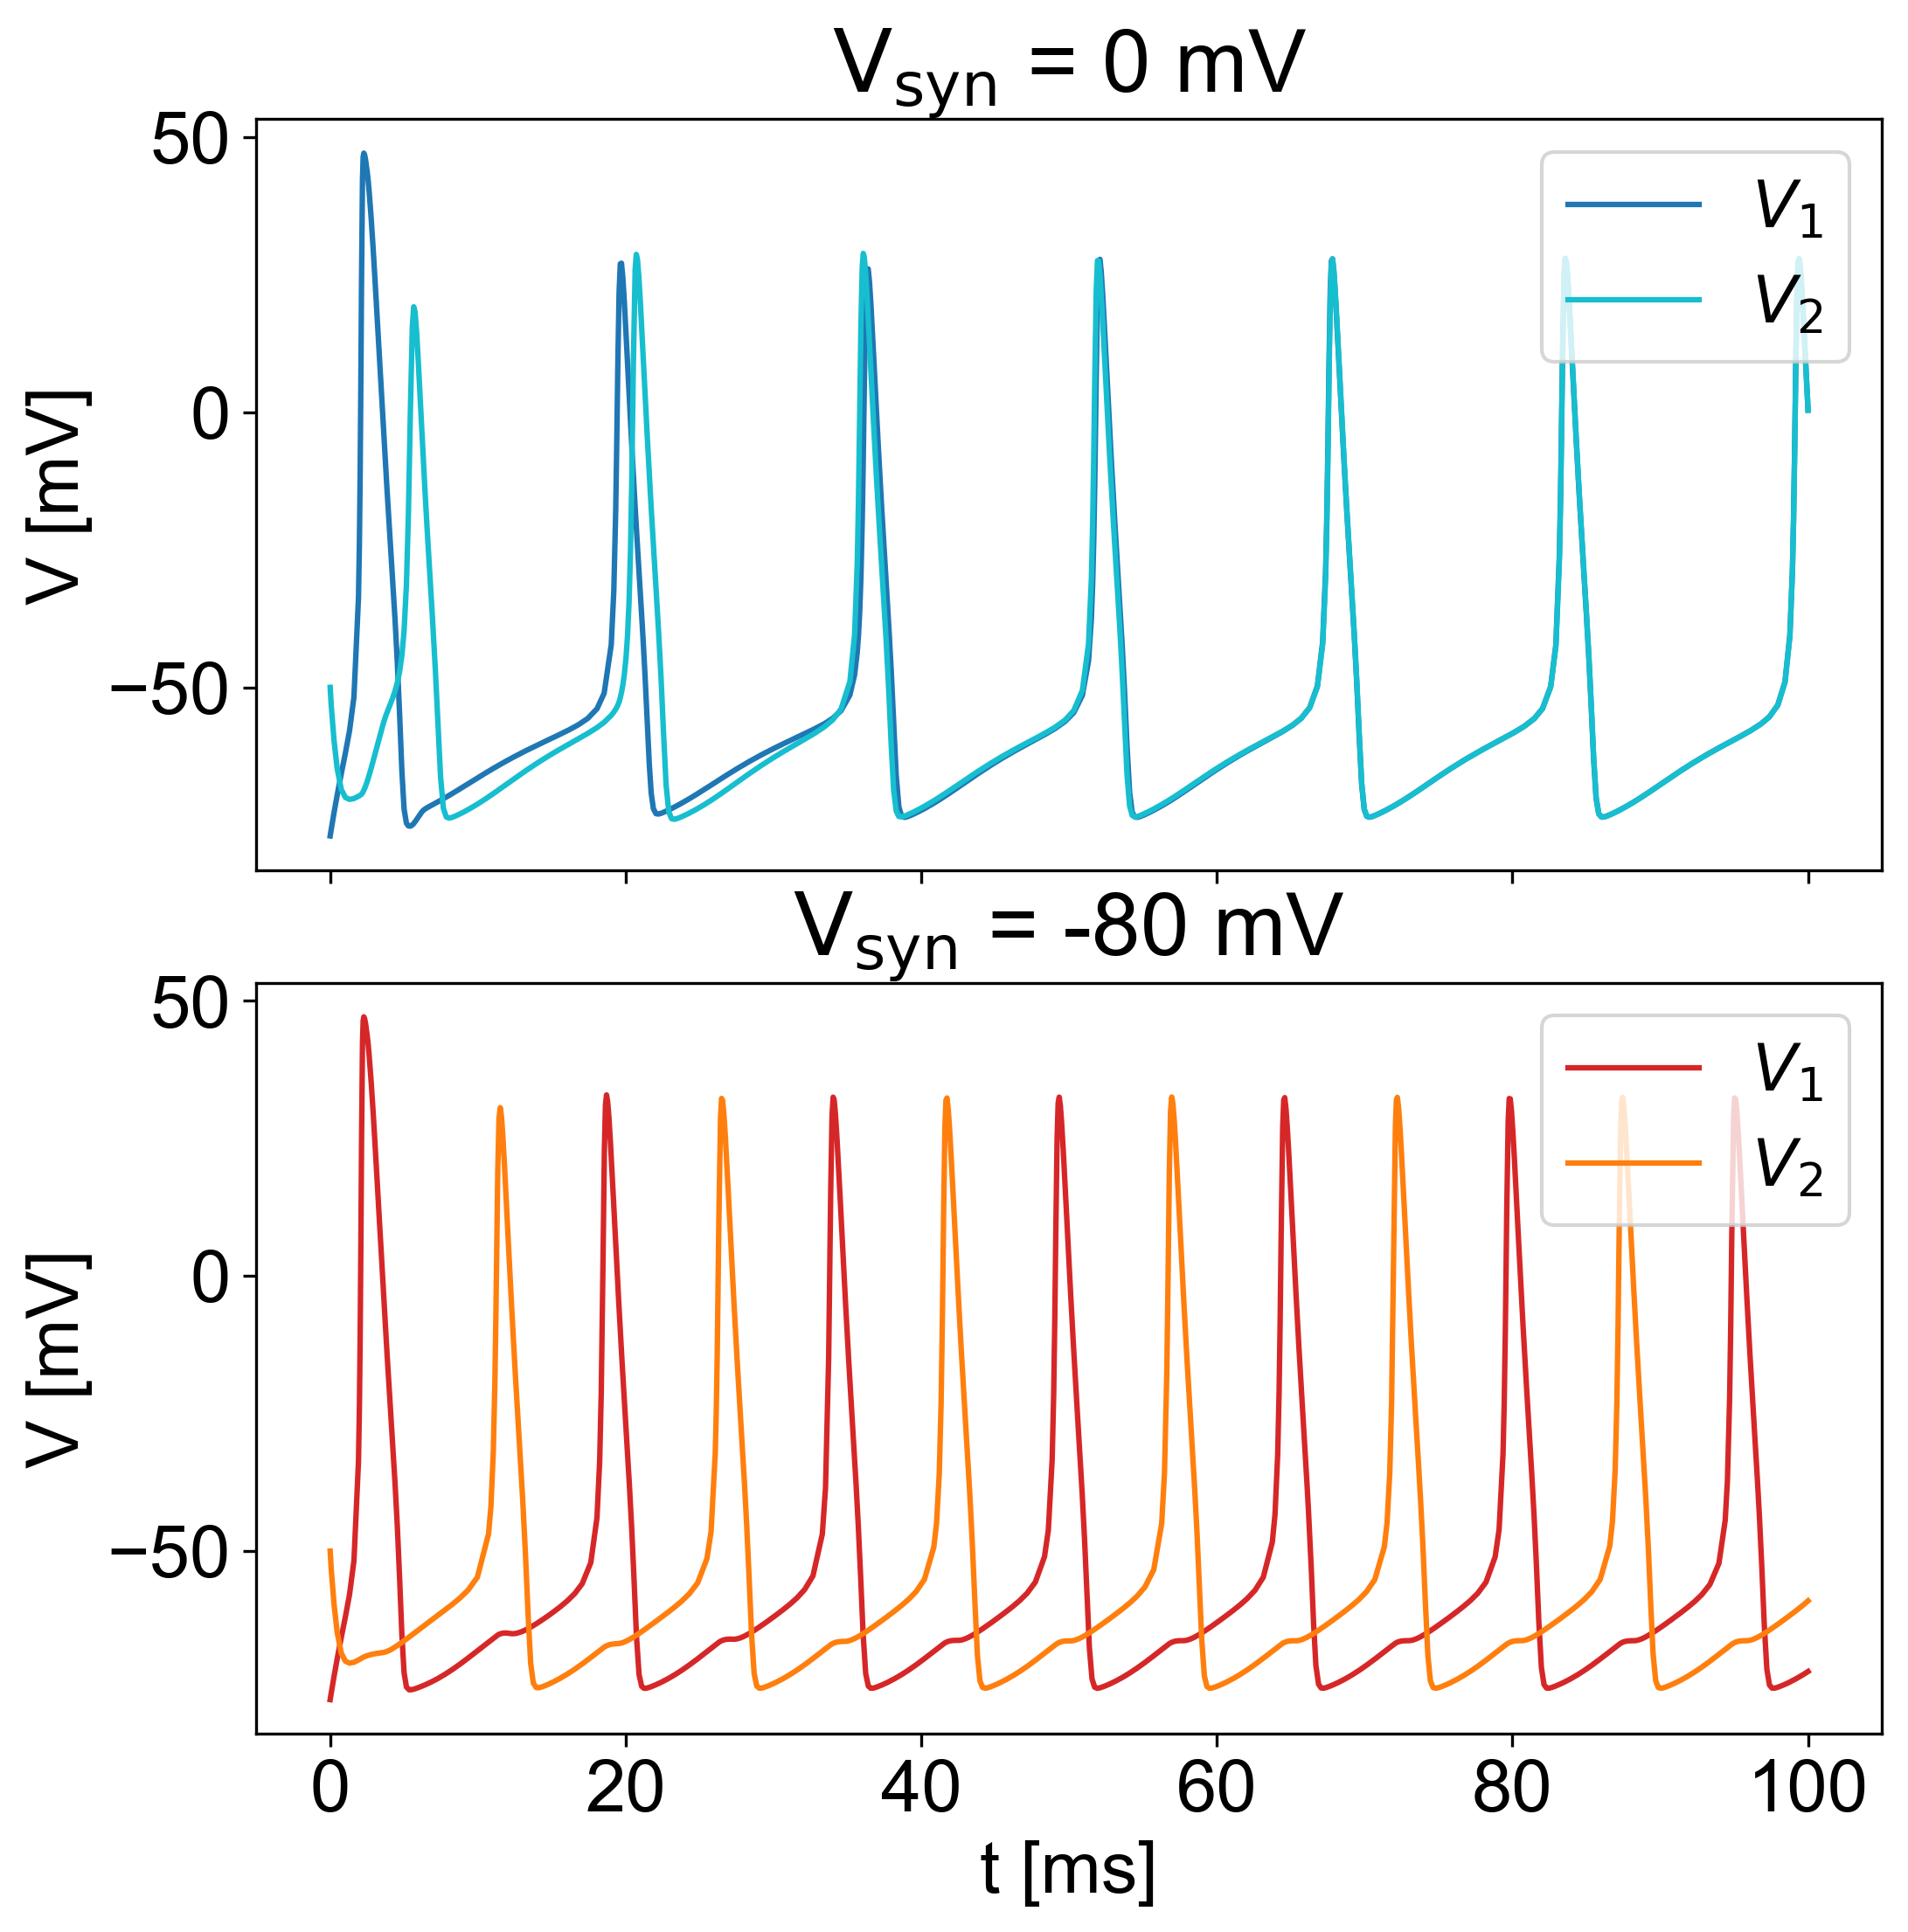
\includegraphics[clip=true,width=\columnwidth]{ej1_potenciales_vs_Vsyn.png}
    \caption{Potenciales de membrana $V_1$ y $V_2$ de ambas neuronas en función del tiempo $t$ para $g_{syn} = 1$ y dos valores distintos de $V_{syn}$.}
    \label{fig:ej1_potenciales_vs_Vsyn}
\end{figure}

Al variar \(g_{syn}\), se observan cambios en la dinámica neuronal. La figura (2) muestra cómo los potenciales varían en el tiempo para diferentes valores de \(g_{syn}\), destacando un cambio en la frecuencia de los spikes con este parámetro.

\begin{figure}[h]
    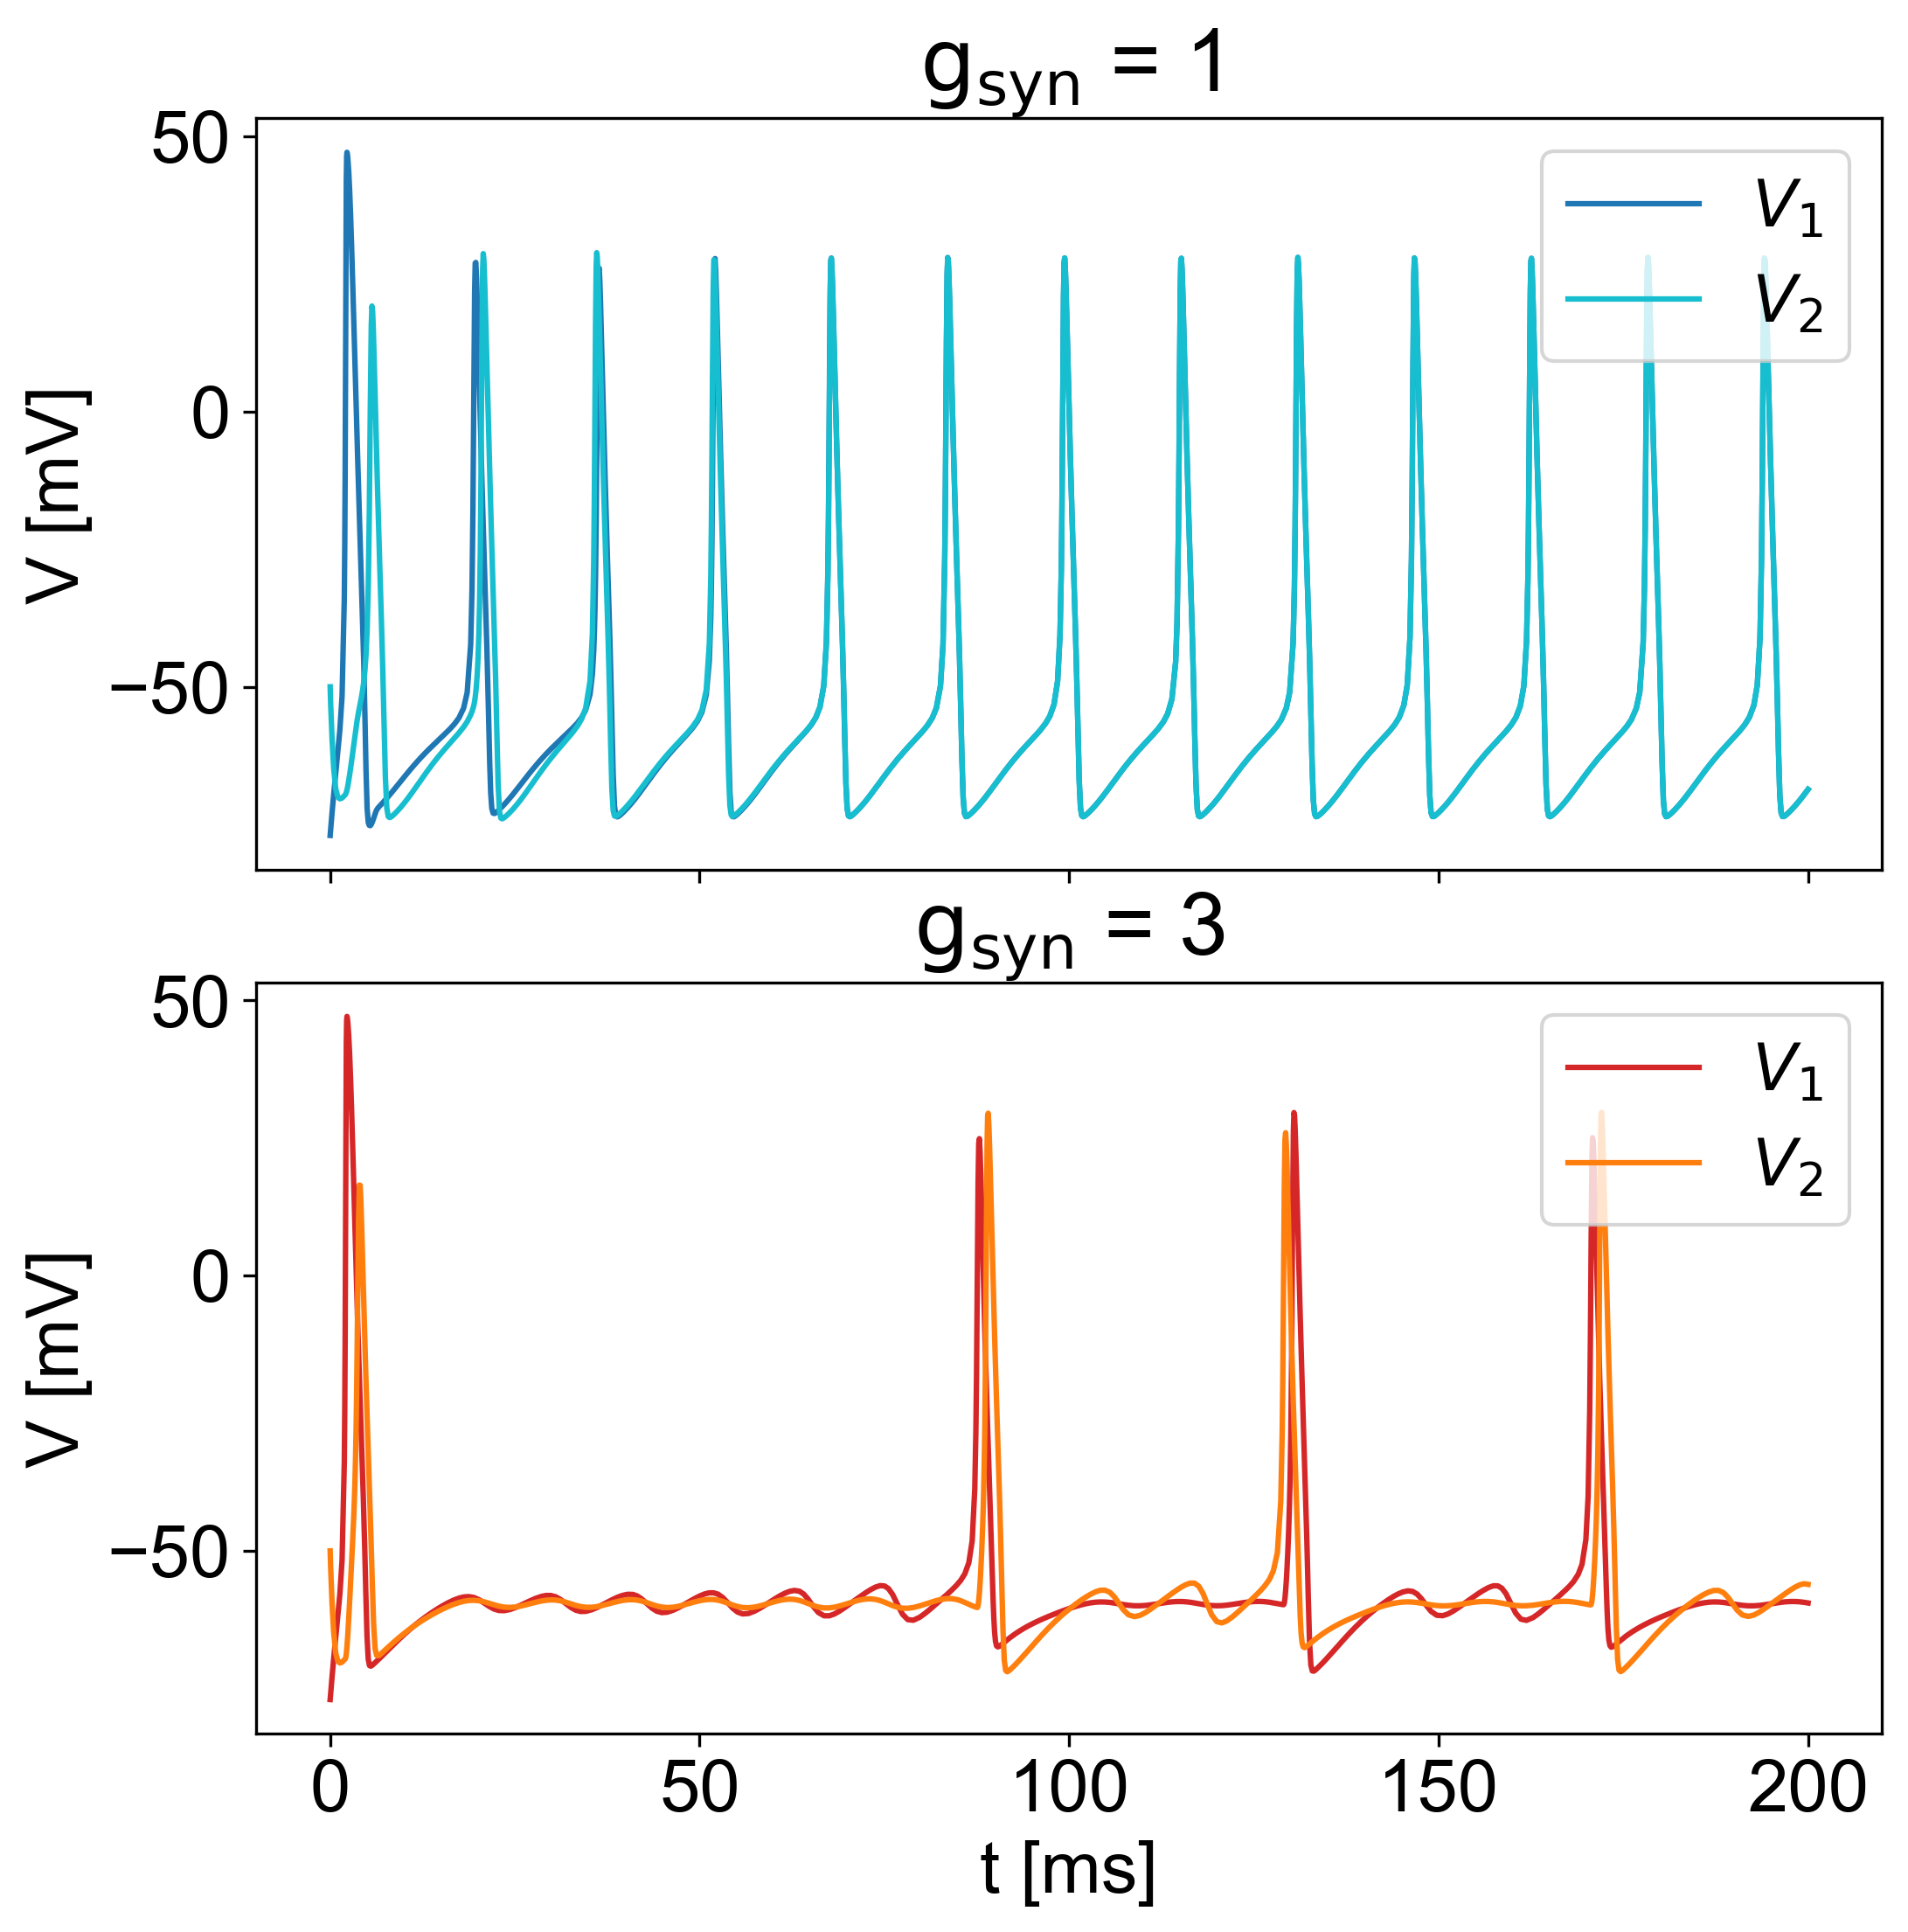
\includegraphics[clip=true,width=\columnwidth]{ej1_potenciales_vs_gsyn.png}
    \caption{Potenciales de membrana $V_1$ y $V_2$ de ambas neuronas en función del tiempo $t$ para $V_{syn} = 0$ y dos valores distintos de $g_{syn}$.}
    \label{fig:ej1_potenciales_vs_gsyn}
\end{figure}

Para describir cuantitativamente los efectos anteriores, se determinó numéricamente la tasa de disparo y el desfasaje entre las neuronas. La tasa de disparo se define como el número de spikes por unidad de tiempo. Mientras que el desfasaje se define como la diferencia temporal entre los picos de ambos potenciales, normalizada por el período del sistema (inverso de la tasa de disparo). Estos cálculos se realizaron en el estado estacionario, después de haber superado la fase transitoria. Todos estos resultados se presentan en la figura (3).


\begin{figure}[h]
   \centering
   \begin{subfigure}[b]{0.45\textwidth}
        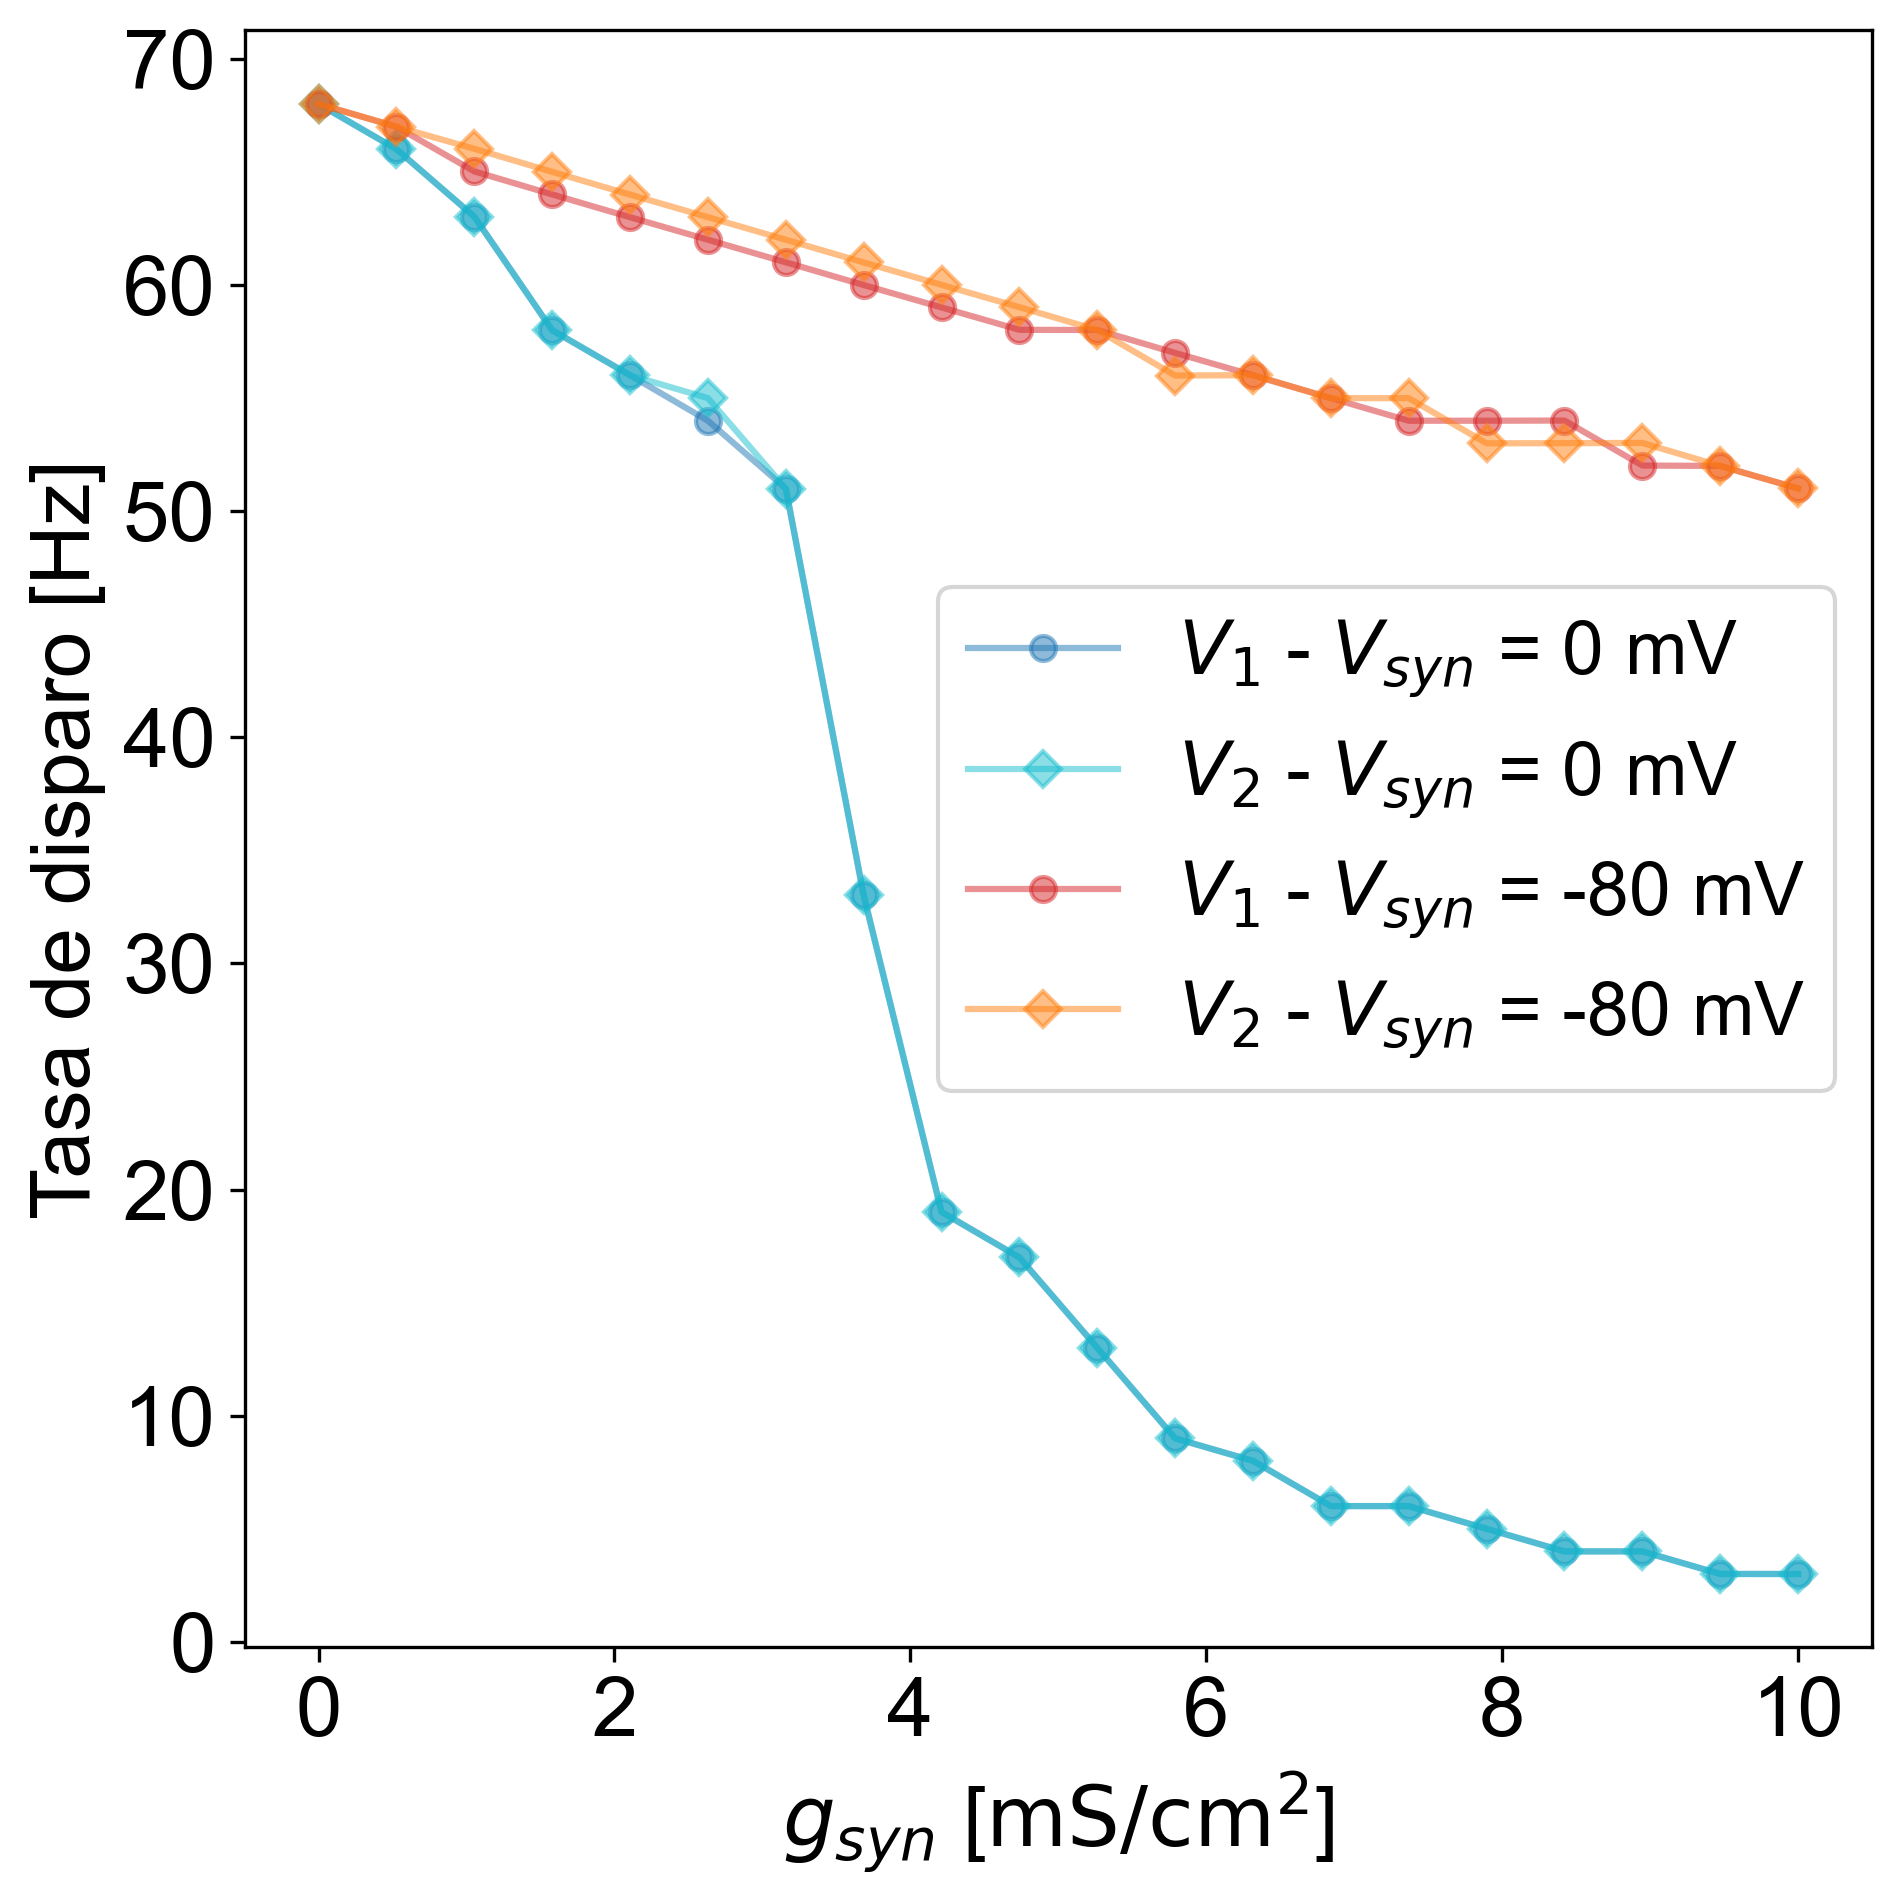
\includegraphics[clip=true,width=\columnwidth]{ej1_tasa.png}
        \caption{\label{fig:ej1_tasa}}
   \end{subfigure}
    \begin{subfigure}[b]{0.45\textwidth}
          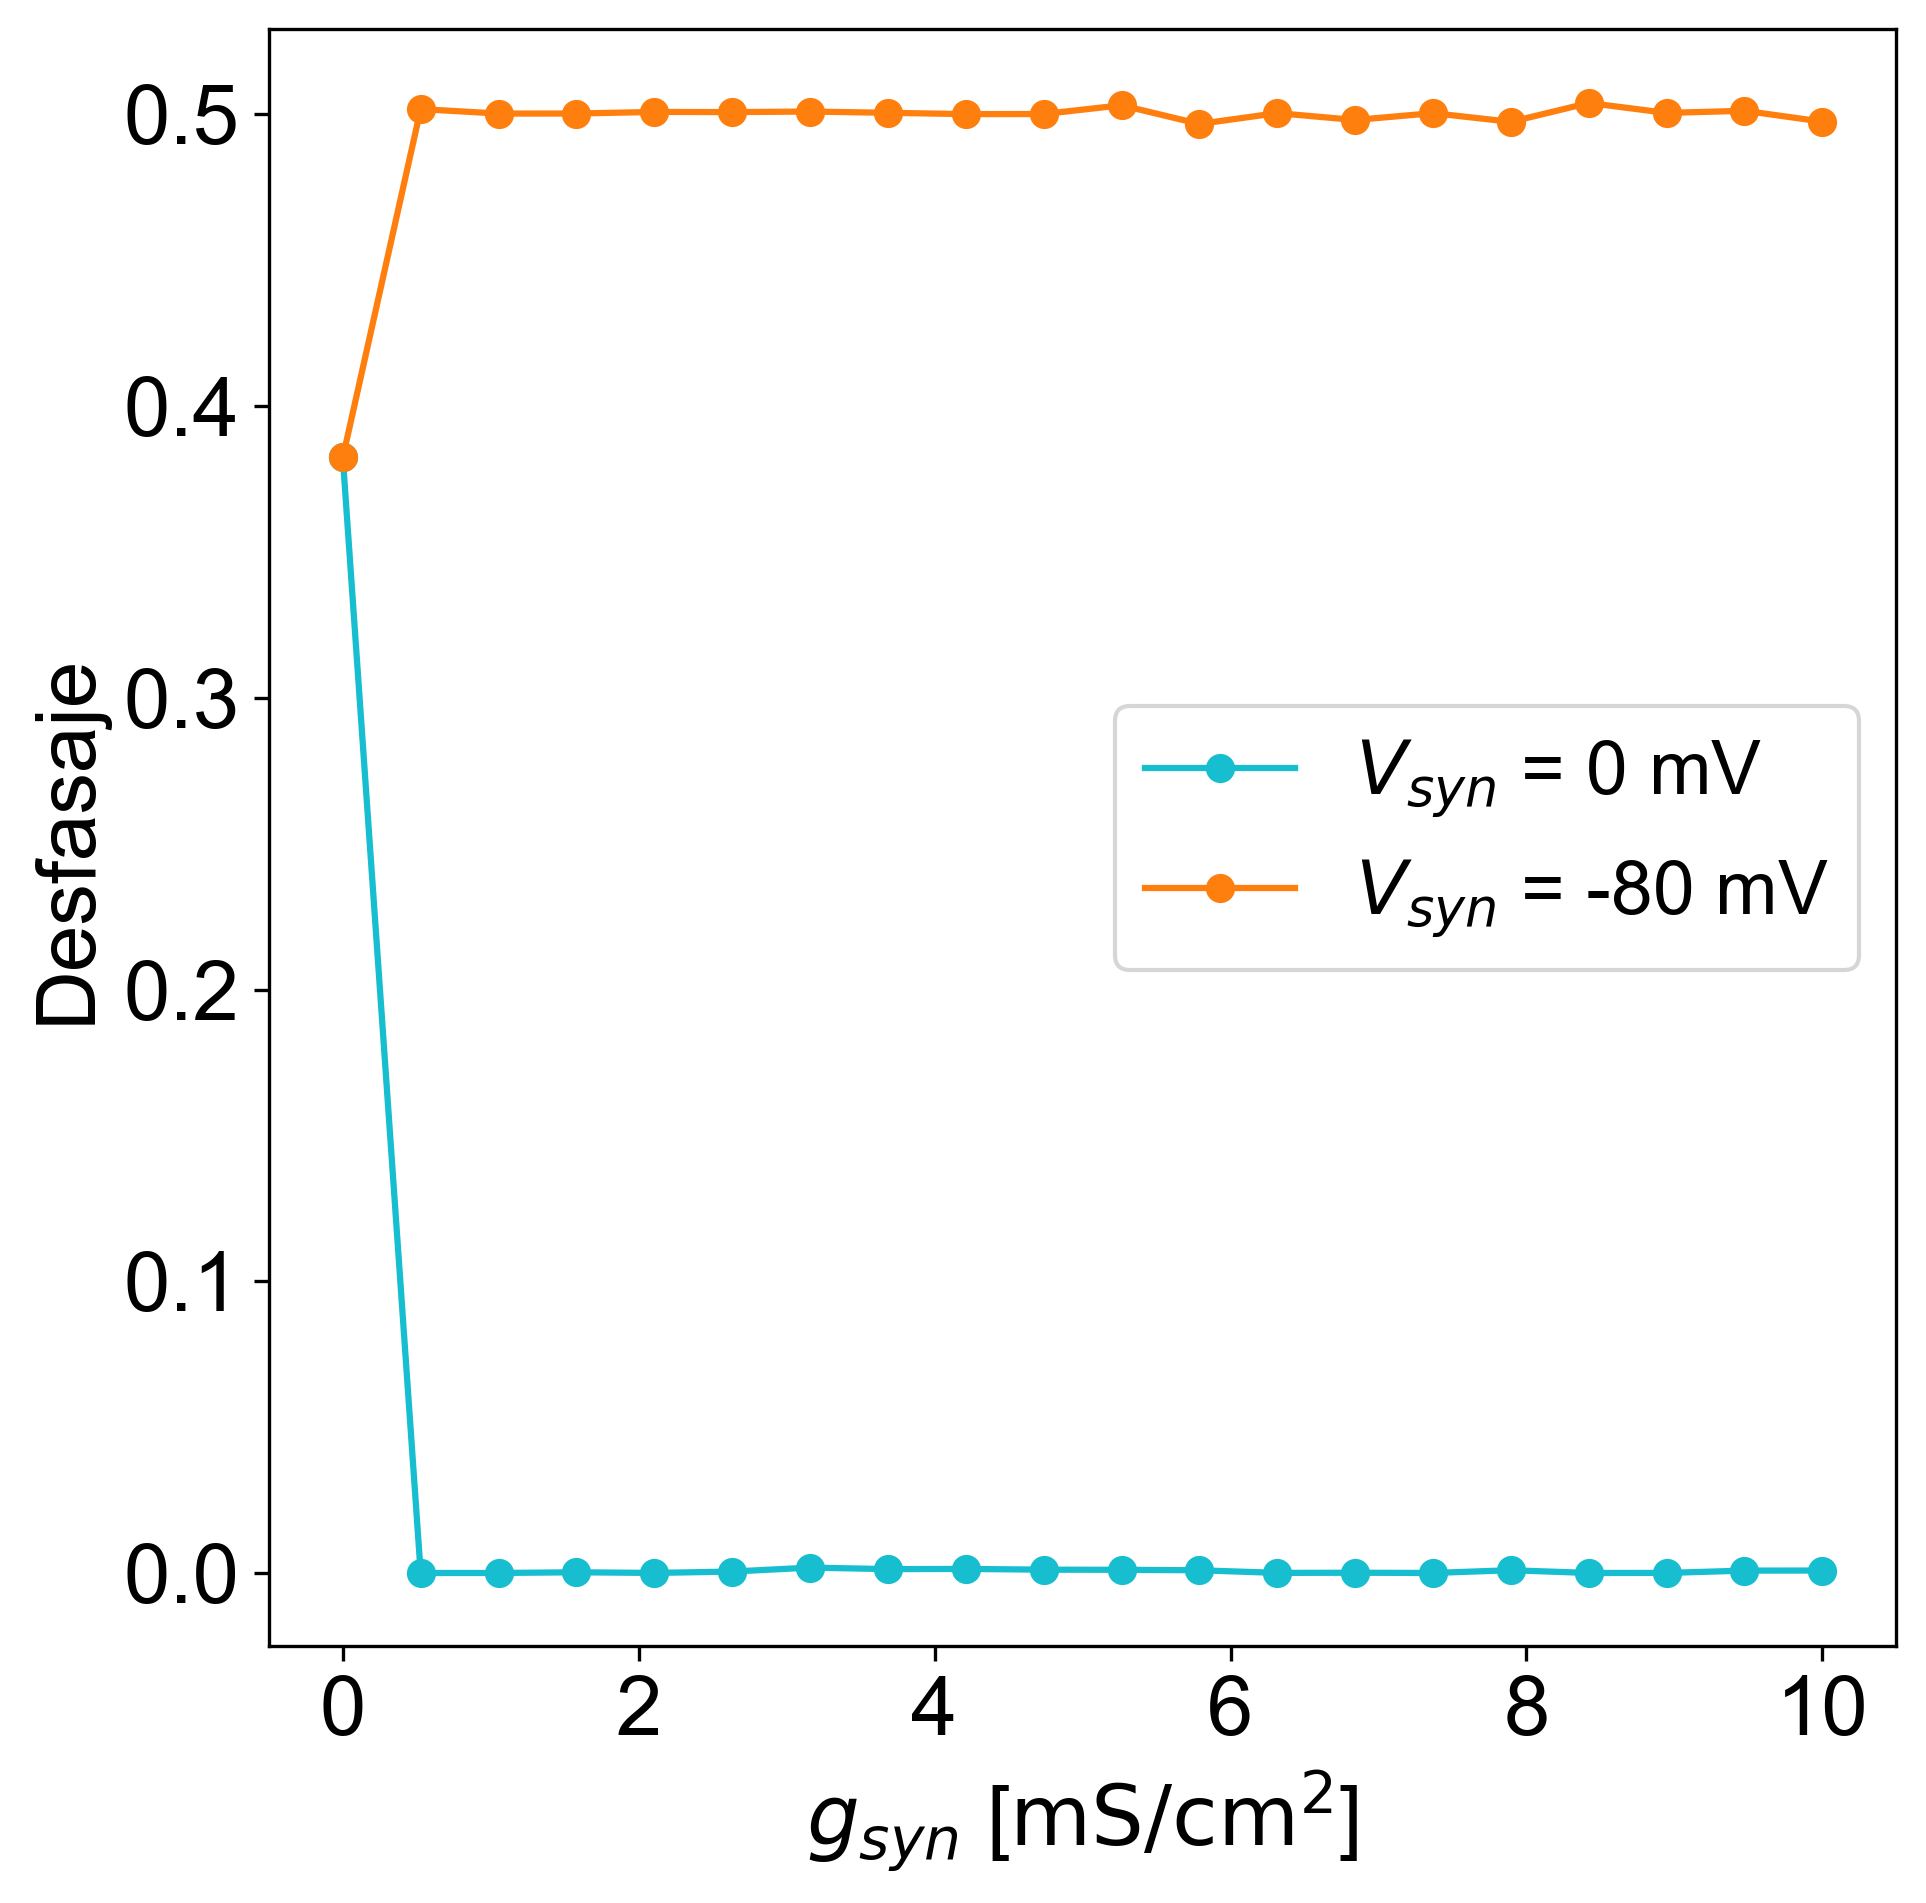
\includegraphics[clip=true,width=\columnwidth]{ej1_desfasaje.png}
          \caption{\label{fig:ej1_desfasaje}}
    \end{subfigure}
    \caption{3.a Tasa de disparo de ambas neuronas y 3.b desfasaje entre neuronas para $V_{syn} = 0$ y $V_{syn} = -80$ mV.}
    \label{fig:ej1_tasa_desfasaje}
\end{figure}




En cuanto a la tasa de disparo, esta disminuye al aumentar \(g_{syn}\) y además disminuye más rápido con una interacción es existatoria. Aunque intuitivamente se esperaría un aumento en la tasa con una mayor interacción, esto no sucede. Una posible explicación es que la corriente de interacción no es constante como $I_{ext}$ y solo actúa en momentos específicos.

En cuanto al desfasaje, con $g_{syn} = 0$, se observa un desfasaje distinto entre las neuronas, lo cual está ligado a la falta de interacción. Sin embargo, para $g_{syn} \neq 0$ el desfasaje parece ser independiente del parámetro, pero totalmente determinado por el tipo de interacción. En interacciones excitatorias, el desfasaje es nulo (comportamiento en fase), mientras que en interacciones inhibitorias, el desfasaje es de 0.5, lo que indica un comportamiento en contrafase.

\section{Ejercicio 2}


Se analizó un sistema compuesto por dos grupos de neuronas: excitatorias e inhibitorias, utilizando el modelo de tasa de disparo (Fire Rate Model). Además, se estableció una relación semilineal entre la frecuencia de disparo y la corriente. Las ecuaciones que describen la dinámica de este sistema son las siguientes

\[
\left\{\begin{array}{@{}l@{}}
    \tau \frac{dh_e}{dt} = -h_e + g_{ee} f_e - g_{ei} f_i + I_e \\
    \tau \frac{dh_i}{dt} = -h_i + g_{ie} f_e - g_{ii} f_i + I_i,
    \end{array}\right.
\]
donde $f_e$ y $f_i$ representan las tasas de disparo, las cuales están relacionadas con el potencial a través de la función semilineal $f_\alpha = f_\alpha(h_\alpha) = h_\alpha\Theta(\alpha)$, con $\Theta(x)$ función de Heaviside. Además, $g_{\alpha \beta}$ indica el peso de acoplamiento entre la población $\alpha$ y la población $\beta$. Si el acoplamiento se dirige a la población de neuronas excitatorias ($e$), el peso es positivo. Mientras que si se dirige a la población de neuronas inhibitorias ($i$), es negativo.

A continuación se estudiará si existe una solución en el estado estacionario en la que ambas poblaciones neuronales muestren actividad distinta de cero y si tal solución es estable.

Para que ambas poblaciones estén activas, las tasas de disparo \(f_e\) y \(f_i\) deben ser mayores que cero. Debido a la relación semilineal con los potenciales, esto implica que \(h_e\) y \(h_i\) también deben ser positivos. En estado estacionario, se presentan dos escenarios:

1. Los potenciales son constantes en el tiempo, lo cual lleva a las ecuaciones:
\[
\left\{\begin{array}{@{}l@{}}
    -h_e + g_{ee} f_e - g_{ei} f_i + I_e = 0 \\
    -h_i + g_{ie} f_e - g_{ii} f_i + I_i = 0.
    \end{array}\right.
\]
    
2. Los potenciales cambian en el tiempo, pero con un comportamiento periódico. En tal caso, es posible integrar las ecuaciones de la dinámica en un período y arribar a las mismas ecuaciones anteriores.

Incorporando la relación entre la tasa de disparo y el potencial y teniendo en cuenta los signos de los pesos, tales ecuaciones se traducen en el sistema algebraico lineal:

\[ A \begin{pmatrix} h_e \\ h_i \end{pmatrix} = - \begin{pmatrix} I_e \\ I_i \end{pmatrix}, \]
donde la matriz \(A\) se define como
\[ A = \begin{pmatrix} |g_{ee}| - 1 & |g_{ei}| \\ |g_{ie}| & |g_{ii}| - 1 \end{pmatrix}. \]
De aquí, se puede deducir
\[ \begin{pmatrix} h_e \\ h_i \end{pmatrix} = - A^{-1} \begin{pmatrix} I_e \\ I_i \end{pmatrix}, \]
con \(A^{-1}\) siendo
\[ A^{-1} = \frac{1}{D} \begin{pmatrix} |g_{ii}| - 1 & -|g_{ei}| \\ -|g_{ie}| & |g_{ee}| - 1 \end{pmatrix} \]
y \(D\) es el determinante de \(A\) dado por
\[D = (|g_{ee}| - 1)(|g_{ii}| - 1) - |g_{ie}||g_{ei}|.\]

En base a lo anterior, para garantizar actividad neuronal es necesario que se cumplan las condiciones:

\[ -\frac{1}{D} [ I_e (|g_{ii}| - 1) - I_i |g_{ei}| ] > 0 \]
\[ -\frac{1}{D} [ -I_e |g_{ie}| + I_i (|g_{ee}| - 1) ] > 0. \]
Por otro lado, la estabilidad de esta solución requiere que la matriz jacobiana del sistema tenga una traza \(T\) negativa y un determinante positivo. Esta matriz coincide con \(\tau A\), estableciendo las condiciones
\[ T = |g_{ee}| + |g_{ii}| - 2 < 0 \]
\[ D = (|g_{ee}| - 1)(|g_{ii}| - 1) - |g_{ie}||g_{ei}| > 0 \]

\onecolumngrid
?
\section{Apéndice}

A continuación se desarrolla el código utilizado en el ejercicio 1 para resolver el sistema de ecuaciones diferenciales acopladas. Este código está implementado en Python

\begin{lstlisting}[language=Python]

    # Práctica 2 - ejercicio 1

# date: 09/09/2023
# File: Chehade_practica2.py
# Author : Pablo Naim Chehade
# Email: pablo.chehade.villalba@gmail.com
# GitHub: https://github.com/Lupama2

#Import libraries
import numpy as np
import matplotlib
import matplotlib.pyplot as plt
from scipy.integrate import solve_ivp
from scipy.signal import find_peaks

#Hago los graficos interactivos
# %matplotlib ipympl

#Fuente y tamaño de los caracteres en los graficos
font = {'family' : 'Arial',
        'weight' : 'normal',
        'size'   : 20}
matplotlib.rc('font', **font)

#########################################################
# PARaMETROS ESTANDAR DEL SISTEMA
#########################################################

C_hat = 1 #[mS]
g_K_adim = 36
g_Na_adim = 120
g_L_adim = 0.3

V_K = -77 #[mV]
V_Na = 50 #[mV]
V_L = -54.4 #[mV]

#########################################################
# FUNCIONES
#########################################################


def m_inf(V):
    a_m = 0.1*(V + 40)/(1 - np.exp(-(V + 40)/10))
    b_m = 4*np.exp(-(V + 65)/18)
    return a_m/(a_m + b_m)

def h_inf(V):
    a_h = 0.07*np.exp(-(V + 65)/20)
    b_h = 1/(1 + np.exp(-(V + 35)/10))
    return a_h/(a_h + b_h)

def n_inf(V):
    a_n = 0.01*(V + 55)/(1 - np.exp(-(V + 55)/10))
    b_n = 0.125*np.exp(-(V + 65)/80)
    return a_n/(a_n + b_n)

def s_inf(V):
    return 0.5*(1 + np.tanh(V/5))

def tau_m(V):
    a_m = 0.1*(V + 40)/(1 - np.exp(-(V + 40)/10))
    b_m = 4*np.exp(-(V + 65)/18)
    return 1/(a_m + b_m)

def tau_h(V):
    a_h = 0.07*np.exp(-(V + 65)/20)
    b_h = 1/(1 + np.exp(-(V + 35)/10))
    return 1/(a_h + b_h)

def tau_n(V):
    a_n = 0.01*(V + 55)/(1 - np.exp(-(V + 55)/10))
    b_n = 0.125*np.exp(-(V + 65)/80)
    return 1/(a_n + b_n)

def tau_s(V):
    return 3

def I_syn(V, s, g_syn, V_syn):
    return - g_syn*s*(V - V_syn)

def tasa_de_disparo(V_signal, t_fin, t_ini):
    '''
    Calcula la tasa de disparo de V
    '''
    peaks, _ = find_peaks(V_signal, height = 0)
    
    #Calculo la tasa de disparo
    tasa = len(peaks)/(t_fin - t_ini)
    return tasa

def desfasaje(t_signal, V1_signal, V2_signal):
    '''
    Calcula el desfasaje entre V1 y V2
    '''
    peaks1, _ = find_peaks(V1_signal, height = 0)
    peaks2, _ = find_peaks(V2_signal, height = 0)
    
    #Determino que picos son consecutivos entre si. Este criterio puedo aplicarlo porque ya conozco como se comporta el problema
    #Determino el primero de los picos
    if peaks1[0] < peaks2[0]:
        #Determino que pico tiene peaks2[0] mas cerca
        if abs(peaks1[0] - peaks2[0]) < abs(peaks1[1] - peaks2[0]):
            peaks1 = peaks1[0:]
        else:
            peaks1 = peaks1[1:]
    else:
        #Determino que pico tiene peaks1[0] mas cerca
        if abs(peaks1[0] - peaks2[0]) < abs(peaks1[0] - peaks2[1]):
            peaks2 = peaks2[0:]
        else:
            peaks2 = peaks2[1:]

    #Calculo el desfasaje como promedio de desfasajes entre picos consecutivos

    desfasajes = np.empty(min(len(peaks1), len(peaks2)))
    for i in range(len(desfasajes)):
        desfasajes[i] = t_signal[peaks1[i]] - t_signal[peaks2[i]]
    
    return np.mean(desfasajes)

def any_vs_g_syn(V_syn, g_syn):
    #Resuelvo sistema de ecuaciones
    t_ini = 0
    t_fin = 2000 #[ms]

    I_ext = 10

    soln = solve_ivp(derivada, [t_ini, t_fin], y0, method = "RK45", args = (I_ext,g_syn,V_syn), dense_output = True)

    #Verifico que se halla resuelto el problema
    if soln.success != True:
        raise ValueError(soln.message)

    #Restrinjo los valores desde que hay un pico en el estacionario
    t_ini_new = t_fin/2
    t_ini_new_ind = np.where(soln.t >= t_ini_new)[0][0]
    #Comienzo a medir desde el primer pico luego de t_ini_new
    peaks_V1, _ = find_peaks(soln.y[0,t_ini_new_ind:], height = 0)
    peaks_V2, _ = find_peaks(soln.y[5,t_ini_new_ind:], height = 0)
    t_ini_new_ind + np.min([peaks_V1[0], peaks_V2[0]])
    t_ini_new = soln.t[t_ini_new_ind]

    #Calculo la tasa de disparo
    tasa_V1 = tasa_de_disparo(soln.y[0,t_ini_new_ind:], t_fin, t_ini_new)
    tasa_V2 = tasa_de_disparo(soln.y[5,t_ini_new_ind:], t_fin, t_ini_new)

    #Calculo el desfasaje
    desfasaje_V1_V2 = desfasaje(soln.t[t_ini_new_ind:], soln.y[0,t_ini_new_ind:], soln.y[5,t_ini_new_ind:])

    return tasa_V1, tasa_V2, desfasaje_V1_V2

#########################################################
# ECUACIONES DIFERENCIALES
#########################################################

def derivada(t, y, I_ext, g_syn, V_syn):
    '''
    C_hat = C / g_hat : [ms = mili segundos]
    I_ext : [muA/cm2]
    V: [mV]
    Derivada
    y[0]: V1
    y[1]: m1
    y[2]: h1
    y[3]: n1
    y[4]: s1
    y[5]: V2
    y[6]: m2
    y[7]: h2
    y[8]: n2
    y[9]: s2
    '''

    #Def derivative vector
    dydt = np.empty(10)
    N_eq = 5 #ec. por neurona

    #Asigno variables
    V1 = y[0]; m1 = y[1]; h1 = y[2]; n1 = y[3]; s1 = y[4]
    V2 = y[5]; m2 = y[6]; h2 = y[7]; n2 = y[8]; s2 = y[9]

    #Eq of charge conservation
    dydt[0] = (1/C_hat) *(I_ext + I_syn(V1, s1, g_syn, V_syn) - g_K_adim*n1**4*(V1 - V_K) - g_Na_adim*m1**3*h1*(V1 - V_Na) - g_L_adim*(V1 - V_L))

    dydt[0 + N_eq] = (1/C_hat) *(I_ext + I_syn(V2, s2, g_syn, V_syn) - g_K_adim*n2**4*(V2 - V_K) - g_Na_adim*m2**3*h2*(V2 - V_Na) - g_L_adim*(V2 - V_L))

    #Eq's m, h, n
    dydt[1] = (m_inf(V1) - m1)/tau_m(V1)
    dydt[2] = (h_inf(V1) - h1)/tau_h(V1)
    dydt[3] = (n_inf(V1) - n1)/tau_n(V1)
    dydt[4] = (s_inf(V2) - s1)/tau_s(V1)

    dydt[1 + N_eq] = (m_inf(V2) - m2)/tau_m(V2)
    dydt[2 + N_eq] = (h_inf(V2) - h2)/tau_h(V2)
    dydt[3 + N_eq] = (n_inf(V2) - n2)/tau_n(V2)
    dydt[4 + N_eq] = (s_inf(V1) - s2)/tau_s(V2)

    return dydt

#########################################################
# CONDICIONES INICIALES
#########################################################

V0_1 = -77
V0_2 = -50

y0_1_vec = np.array([V0_1, m_inf(V0_1), h_inf(V0_1), n_inf(V0_1), s_inf(V0_1)])
y0_2_vec = np.array([V0_2, m_inf(V0_2), h_inf(V0_2), n_inf(V0_2), s_inf(V0_2)])

y0 = np.concatenate((y0_1_vec, y0_2_vec))

#########################################################
# V1 y V2 vs V_syn
#########################################################

#Grafico para ambos V_syn

t_ini = 0
t_fin = 100 #[ms]

I_ext = 10
g_syn = 1#0.5#2.564102564102564#1
V_syn_1 = 0
V_syn_2 = -80

soln_1 = solve_ivp(derivada, [t_ini, t_fin], y0, method = "RK45", args = (I_ext,g_syn,V_syn_1), dense_output = True)
soln_2 = solve_ivp(derivada, [t_ini, t_fin], y0, method = "RK45", args = (I_ext,g_syn,V_syn_2), dense_output = True)

#Verifico que se halla resuelto el problema
if soln_1.success != True or soln_2.success != True:
    raise ValueError(soln_1.message)

#Grafico
fig, ax = plt.subplots(2,1, sharex=True, figsize = (8,8))
#Junto mas los subplots
fig.subplots_adjust(hspace=0.15)

ax[0].plot(soln_1.t, soln_1.y[0,:], label = "$V_1$", color = "tab:blue")
ax[0].plot(soln_1.t, soln_1.y[5,:], label = "$V_2$", color = "tab:cyan")
ax[0].set_title("$\mathrm{V_{syn}}$ = 0 mV")
# ax[0].set_xlabel("t [ms]")
ax[0].set_ylabel("V [mV]")
ax[0].legend(fontsize = 18, loc = "upper right")

ax[1].plot(soln_2.t, soln_2.y[0,:], label = "$V_1$", color = "tab:red")
ax[1].plot(soln_2.t, soln_2.y[5,:], label = "$V_2$", color = "tab:orange")
ax[1].set_title("$\mathrm{V_{syn}}$ = -80 mV")
ax[1].set_xlabel("t [ms]")
ax[1].set_ylabel("V [mV]")
ax[1].legend(fontsize = 18, loc = "upper right")

plt.show()

#Guardo imagen
# fig.savefig("Informe/ej1_potenciales_vs_Vsyn.png", dpi = 300, bbox_inches = "tight")

#########################################################
# V1 y V2 vs g_syn
#########################################################

#Grafico para  dos alores de g_syn

t_ini = 0
t_fin = 200 #[ms]

I_ext = 10
g_syn_1 = 1 #0.5#2.564102564102564#1
g_syn_2 = 4
V_syn = 0

soln_1 = solve_ivp(derivada, [t_ini, t_fin], y0, method = "RK45", args = (I_ext,g_syn_1,V_syn), dense_output = True)
soln_2 = solve_ivp(derivada, [t_ini, t_fin], y0, method = "RK45", args = (I_ext,g_syn_2,V_syn), dense_output = True)

#Verifico que se halla resuelto el problema
if soln_1.success != True or soln_2.success != True:
    raise ValueError(soln_1.message)

#Grafico
fig, ax = plt.subplots(2,1, sharex=True, figsize = (8,8))
#Junto mas los subplots
fig.subplots_adjust(hspace=0.15)

ax[0].plot(soln_1.t, soln_1.y[0,:], label = "$V_1$", color = "tab:blue")
ax[0].plot(soln_1.t, soln_1.y[5,:], label = "$V_2$", color = "tab:cyan")
ax[0].set_title("$\mathrm{g_{syn}}$ = 1")
# ax[0].set_xlabel("t [ms]")
ax[0].set_ylabel("V [mV]")
ax[0].legend(fontsize = 18, loc = "upper right")

ax[1].plot(soln_2.t, soln_2.y[0,:], label = "$V_1$", color = "tab:red")
ax[1].plot(soln_2.t, soln_2.y[5,:], label = "$V_2$", color = "tab:orange")
ax[1].set_title("$\mathrm{g_{syn}}$ = 3")
ax[1].set_xlabel("t [ms]")
ax[1].set_ylabel("V [mV]")
ax[1].legend(fontsize = 18, loc = "upper right")

plt.show()

#Guardo imagen
# fig.savefig("Informe/ej1_potenciales_vs_gsyn.png", dpi = 300, bbox_inches = "tight")

#########################################################
# TASA DE DISPARO y DESFASAJE vs g_syn
#########################################################
V_syn = 0

N = 20
g_syn_vec = np.linspace(0,10, num = N)

any_vs_g_syn_vec = np.empty([N, 3])

for i in range(N):
    print("Calculo: ", i+1, " de ", N)
    any_vs_g_syn_vec[i] = any_vs_g_syn(V_syn, g_syn_vec[i])

#Guardo datos como .npy
data_1 = np.vstack([g_syn_vec, any_vs_g_syn_vec.T])
# file_name = f"data_V_syn_{V_syn:.2f}.npy"
# np.save(file_name, data)

V_syn = -80

N = 20
g_syn_vec = np.linspace(0,10, num = N)

any_vs_g_syn_vec = np.empty([N, 3])

for i in range(N):
    print("Calculo: ", i+1, " de ", N)
    any_vs_g_syn_vec[i] = any_vs_g_syn(V_syn, g_syn_vec[i])

#Guardo datos como .npy
data_2 = np.vstack([g_syn_vec, any_vs_g_syn_vec.T])
# file_name = f"data_V_syn_{V_syn:.2f}.npy"
# np.save(file_name, data)


#Cargo datos
# data_1 = np.load("data_V_syn_0.00.npy")
# data_2 = np.load("data_V_syn_-80.00.npy")

#Desempaqueto y grafico
g_syn_vec_1, any_vs_g_syn_vec_1 = data_1[0], data_1[1:].T
g_syn_vec_2, any_vs_g_syn_vec_2 = data_2[0], data_2[1:].T

factor_ms_to_s = 1000

fig, ax = plt.subplots(1,1, figsize = (7,7))

ax.plot(g_syn_vec_1, any_vs_g_syn_vec_1[:,0]*factor_ms_to_s, "o-", label = r"$V_1$ - $V_{syn}$ = 0 mV", alpha = 0.5, color = "tab:blue")
ax.plot(g_syn_vec_1, any_vs_g_syn_vec_1[:,1]*factor_ms_to_s, "D-", label = r"$V_2$ - $V_{syn}$ = 0 mV", alpha = 0.5, color = "tab:cyan")
ax.plot(g_syn_vec_1, any_vs_g_syn_vec_2[:,0]*factor_ms_to_s, "o-", label = r"$V_1$ - $V_{syn}$ = -80 mV", alpha = 0.5, color = "tab:red")
ax.plot(g_syn_vec_1, any_vs_g_syn_vec_2[:,1]*factor_ms_to_s, "D-", label = r"$V_2$ - $V_{syn}$ = -80 mV", alpha = 0.5, color = "tab:orange")

ax.set_xlabel("$g_{syn}$ [$\mathrm{mS/cm^2}$]")
ax.set_ylabel("Tasa de disparo [Hz]")
#Ubico leyenda abajo a la izquierda
#Cambio el tamaño de la leyenda
ax.legend(fontsize = 18)
plt.show()

#Guardo imagen
fig.savefig("Informe/ej1_tasa.png", dpi = 300, bbox_inches = "tight")

fig, ax = plt.subplots(1,1, figsize = (7,7))

tasa_de_disparo_mean_1 = (any_vs_g_syn_vec_1[:,0] + any_vs_g_syn_vec_1[:,1])/2
tasa_de_disparo_mean_2 = (any_vs_g_syn_vec_2[:,0] + any_vs_g_syn_vec_2[:,1])/2

ax.plot(g_syn_vec_1, np.abs(any_vs_g_syn_vec_1[:,2])*tasa_de_disparo_mean_1, "o-", label = "$V_{syn}$ = 0 mV", color = "tab:cyan")
ax.plot(g_syn_vec_2, np.abs(any_vs_g_syn_vec_2[:,2])*tasa_de_disparo_mean_2, "o-", label = "$V_{syn}$ = -80 mV", color = "tab:orange")

ax.set_xlabel("$g_{syn}$ [$\mathrm{mS/cm^2}$]")
ax.set_ylabel("Desfasaje")
ax.legend(fontsize = 18)
plt.show()

#Guardo imagen
# fig.savefig("Informe/ej1_desfasaje.png", dpi = 300, bbox_inches = "tight")

\end{lstlisting}
    

% \bibliography{Chehade_practica_2.bib}

\end{document}





